\documentclass[journal]{IEEEtran}
\usepackage[a5paper, margin=10mm, onecolumn]{geometry}
\usepackage{amsmath,amssymb,amsfonts,amsthm}
\usepackage{gvv-book}
\usepackage{gvv}
\usepackage{hyperref}

\begin{document}

\title{2.4.43}
\author{Puni Aditya - EE25BTECH11046}
\maketitle

\textbf{Question:}\\
Show that the lines $\frac{x-5}{7}=\frac{y+2}{-5}=\frac{z}{1}$ and $\frac{x}{1}=\frac{y}{2}=\frac{z}{3}$ are perpendicular to each other.

\textbf{Solution:}\\
Let the two given lines be $L_1$ and $L_2$.
\begin{align*}
    L_1: \frac{x-5}{7} = \frac{y+2}{-5} = \frac{z}{1} \\
    L_2: \frac{x}{1} = \frac{y}{2} = \frac{z}{3}
\end{align*}
The direction vector of a line in the form $\frac{x-x_1}{a} = \frac{y-y_1}{b} = \frac{z-z_1}{c}$ are
\begin{align*}
\vec{d} = \myvec{a \\ b \\ c}
\end{align*}

Let the direction vector of lines $L_1$ and $L_2$ be $\vec{d_1}$ and $\vec{d_2}$.
From the equations of the lines $L_1$ and $L_2$,
\begin{align}
    \vec{d_1} = \myvec{7 \\ -5 \\ 1}, 
    \vec{d_2} = \myvec{1 \\ 2 \\ 3}
\end{align}

For the two lines to be perpendicular, the inner product or dot product of their direction vectors must be zero.
\begin{align}
    \vec{d_1}^\top \vec{d_2} = 0 \label{eq:1}
\end{align}
\begin{align}
    \vec{d_1}^\top \vec{d_2} &= \myvec{7&-5&1} \myvec{1 \\ 2 \\ 3} \\
    &= \brak{7}\brak{1} + \brak{-5}\brak{2} + \brak{1}\brak{3} \\
    &= 7 - 10 + 3 \\
    &= 0
\end{align}

$\because$ The dot product of the direction vectors of the two lines is 0 \\
$\implies$ The lines are \textbf{perpendicular} to each other.

\begin{figure}
    \centering
    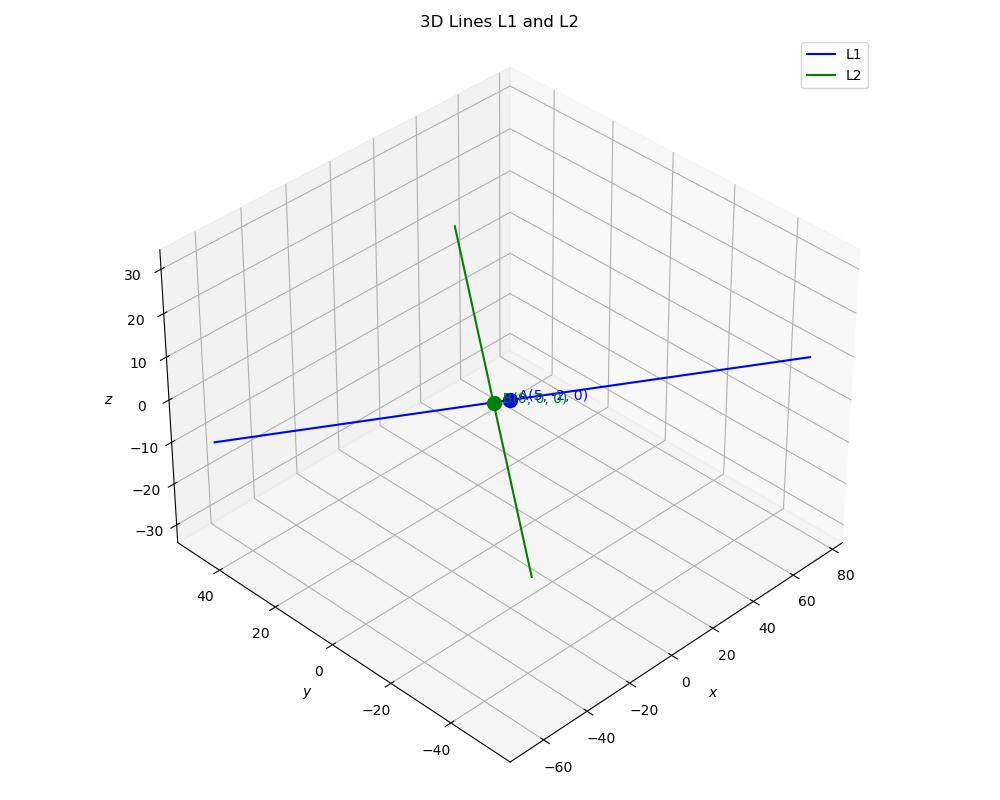
\includegraphics[width=\columnwidth]{figs/plot_c.jpg}
    \caption*{Lines $L_1$ and $L_2$}
    \label{fig:fig}
\end{figure}

\end{document}
